% !TeX program = lualatex
% !TeX root = luaking.tex
% !TeX encoding = UTF-8
% !TeX spellcheck = cs_CZ
%---------------------------------------------------------------------------------------------------
% file fey1ch06.tex
\graphicspath{{../src/FYZ/img/}}
%---------------------------------------------------------------------------------------------------
%================= Kapitola: Pravděpodobnost =======================================================
\setchaptertoc
\chapter{Feynmanova přednáška o pravděpodobnosti}\label{chap:fey_ppst}
\epigraph{\emph{The true logic of this world is in the calculus of probabilities.}}{James Clerk 
Maxwell}
  \section{Možnost a pravděpodobnost}
    Možnost je slovo, které se často používá v každodenním životě. V rozhlasovém zpravodajství o 
    zítřejším počasí můžeme slyšet: „Zítra odpoledne předpovídáme možnost bouřek.“ Můžeme si říci: 
    „Mám jen malou možnost dožít se sta let.“ I vědci používají slovo možnost. Seismologové si 
    kladou otázku: Jaká je možnost, že v příštím roce bude v jižní Kalifornii zemětřesení určité 
    intenzity?“ Fyzik si může položit otázku: Jaká je možnost, že určitý Geigerův počítač 
    zaregistruje v příštích \num{10} sekundách \num{20} částic?“ Politika nebo státníka může 
    zajímat otázka: Jaká je možnost, že v průběhu následujících deseti let dojde k jaderné válce?“ 
    Vás může zajímat, jakou máte možnost se něco naučit z této kapitoly.
    
    \emph{Možností} rozumíme něco jako odhad. Proč odhadujeme? Odhady děláme tehdy, když chceme 
    něco posoudit, ale máme neúplné informace nebo nespolehlivé znalosti. Chceme uhádnout, jaké 
    věci jsou, nebo co se stane. Často také děláme odhad před nějakým rozhodnutím. Například: Mám 
    si vzít zítra plášť do deště? S jakým pohybem půdy bych měl počítat při návrhu nové stavby? Mám 
    si vybudovat protiatomový kryt? Mám změnit své stanovisko při mezinárodních jednáních? Mám dnes 
    jít do školy?
    
    Někdy děláme odhad proto, že se svými omezenými znalostmi chceme co nejvíce říci o určité 
    situaci. V odhadu je skutečně velké zobecnění. Jakákoli fyzikální teorie je jistým druhem 
    odhadu. Existují dobré a špatné odhady. Teorie pravděpodobnosti představuje systém pro     
    vytváření co nejlepších odhadů. Řeč pravděpodobnosti nám dovoluje hovořit kvantitativně o 
    určitých situacích, jež mohou být velmi proměnlivé, ale které mají určité stálé průměrné 
    chování.
    
    Uvažujme házení mincí. Jsou-li samotný hod i mince „poctivé“, nemůžeme vědět, jaký bude 
    výsledek určitého jednotlivého hodu. Přece však cítíme, že při velkém počtu hodů budou 
    přibližně stejně zastoupeny hlavy i znaky. Proto říkáme: „Pravděpodobnost, že padne hlava, je 
    \num{0.5}.“
    
    O pravděpodobnosti hovoříme jen při takových pozorováních, o nichž předpokládáme, že se 
    uskuteční v budoucnosti. \emph{„Pravděpodobnosti“ určitého výsledku pozorováni rozumíme náš 
    odhad toho, jaká část z velkého počtu provedených pozorováni nejspíše dá tento očekávaný 
    výsledek}. Představíme-li si, že pozorování - takové jako pohled na právě hozenou minci - se 
    opakuje \(N\)- krát a označíme-li \(N_A\) \emph{náš odhad} počtu těch pozorování, která dávají 
    určitý výsledek \(A\) (řekněme hlavu), pak pravděpodobností \(P (A)\) pozorování \(A\) rozumíme
    \begin{equation}\label{fyz:eq069}
      P(A) = \frac{N_A}{N}.
    \end{equation}
    
    Naše definice si vyžaduje několik poznámek. O pravděpodobnosti nějaké události můžeme hovořit 
    jen tehdy, je-li tato možným výsledkem nějakého \emph{opakovatelného} pozorování. Není jasné, 
    má-li smysl se ptát: Jaká je pravděpodobnost toho, že v tomto domě straší?“
    
    Mohli bychom namítat, že žádná situace není přesně opakovatelná. To je pravda. Každé další 
    pozorování provádíme přinejmenším v jiném čase nebo na jiném místě. Můžeme říci jen tolik, že 
    „opakovaná“ pozorování by se měla v souladu s naším záměrem \emph{jevit jako ekvivalentní}. 
    Měli bychom předpokládat alespoň to, že každé pozorování se provádělo ve stejně připravené 
    situaci a zejména se stejným stupněm nevědomosti na počátku. (Jestliže se nám podaří nahlédnout 
    do soupeřových karet, bude odhad naděje našeho vítězství jiný než v případě, kdy jsme soupeřovy 
    karty neviděli!)
    
    Je třeba zdůraznit, že \(N\) a \(N_A\) ve vztahu (\ref{fyz:eq069}) \emph{nechápeme} jako čísla 
    založená na skutečných pozorováních. \(N_A\) je náš nejlepší \emph{odhad} toho, co \emph{by 
    mělo} nastat při \(N\) \emph{myšlených} pozorováních. Pravděpodobnost proto závisí na našich 
    znalostech a na naší schopnosti odhadovat. Závisí na našem úsudku! Lidé naštěstí uvažují o 
    mnoha věcech do určité míry stejně, a tak i jejich odhad bude stejný. Pravděpodobnosti však 
    nemusejí být „absolutními“ čísly. Protože závisí na naší nevědomosti, mohou se změnit se změnou 
    našich poznatků.
    
    Možná jsme si všimli jiného, dost „subjektivního“ aspektu naší definice pravděpodobnosti. 
    Hovořili jsme o \(N_A\) jako o „našem odhadu toho, jaká část pozorování nejspíše povede...“. 
    Nerozumíme tím, že budeme pozorovat přesně hodnotu \(N_A\), ale že očekáváme číslo blízké 
    \(N_A\), a že to číslo \(N_A\) je \emph{pravděpodobnější} než jiná čísla v sousedství. 
    Hodíme-li minci \num{30}-krát, neočekáváme, že počet hlav bude přesně \num{15}, ale že to bude 
    spíše nějaké jiné číslo blízké \num{15}, např. \num{12}, \num{13}, \num{14}, \num{15}, \num{16} 
    nebo \num{17}. Jestliže se však musíme pro nějaké číslo rozhodnout, pak si zvolíme \num{15} 
    jako nejpravděpodobnější počet hlav. Můžeme psát \(P(hlava) = \num{0.5}\).
    
    Proč jsme se rozhodli pro \num{15} jako pro nejpravděpodobnější Číslo? V duchu jsme měli 
    následující důvody: Když z celkového počtu hodů \(N\) je \(N_H\) nejpravděpodobnější počet 
    hlav, pak nejpravděpodobnější počet znaků je \((N - N_H)\). (Předpokládáme, že každý hod dá 
    buď hlavu \emph{nebo} znak a jiná možnost neexistuje!) Je-li však mince „poctivá“, není důvodu 
    pro upřednostnění hlav před znaky. Pokud není důvod pro předpoklad nepoctivosti mince (nebo 
    hodu), musíme výskyt hlavy považovat za stejně pravděpodobný jako výskyt znaku. Musíme tedy 
    položit \(N_Z = N_H\). Pak platí
    \begin{equation}\label{fyz:eq070}
      N_Z = N_H = \frac{1}{2} \quad \text{nebo}\quad P(H) = P(Z) = \num{0.5}.
    \end{equation}
    
    Naši argumentaci můžeme zobecnit na \emph{jakoukoli} situaci, v níž existuje \(m\) různých, ale 
    ekvivalentních, tj. stejně možných výsledků pozorování. Může-li pozorování vést k \(m\) různým 
    výsledkům a máme důvod věřit, že každý z nich je stejně možný jako jiný, pak pravděpodobnost 
    \emph{příslušného} výsledku \(A\) je
    \begin{equation}\label{fyz:eq071}
      P(A) = \frac{1}{m}.
    \end{equation}
    
    Je-li v neprůhledné krabici sedm kuliček různých barev a jednu náhodně vybereme (aniž bychom se 
    na ně podívali), je pravděpodobnost vytažení určité barvy \num{1/7}. Pravděpodobnost, že ze 
    zamíchané hromady \num{52} karet „naslepo“ vytáhneme právě srdcové eso je rovna \num{1/52}. 
    Pravděpodobnost hodu dvojnásobné jednotky při hře v kostky je \num{1/36}.
    
    V kapitole \ref{Vol02:fyz:IchapV} jsme popisovali velikost jádra pomocí jeho zdánlivé plochy
    neboli „průřezu“. Přitom jsme vlastně hovořili o pravděpodobnostech. Když ostřelujeme tenkou
    vrstvu materiálu vysokoenergetickými částicemi, existuje jistá naděje, že částice projde
    materiálem a jistá naděje, že narazí na jádro. (Protože jádro je tak malé, že ho nemůžeme vidět,
    nemůžeme na něj přímo mířit. Musíme střílet „naslepo“.) Je-li v naší vrstvě materiálu \(n\)
    atomů a jádro každého atomu má plochu průřezu \(\sigma\), pak celková plocha „zastíněná“ jádry
    je \(n\sigma\). Při velkém počtu \(N\) náhodných střel očekáváme, že počet nárazů \(N_C\) do
    \emph{některého} jádra bude v takovém poměru k \(N\), jaký je poměr zastíněné plochy k celkové
    ploše vrstvy
    \begin{equation}\label{fyz:eq072}
      \frac{N_C}{N} = \frac{n\sigma}{A}.
    \end{equation}
    Je proto možné říci, že pravděpodobnost srážky letící částice při průchodu vrstvou je
    \begin{equation}\label{fyz:eq073}
      P_C = \frac{n}{A}\sigma.
    \end{equation}
    kde \(\frac{n}{A}\) je počet atomů v jednotkové ploše vrstvy.
    
  \section{Fluktuace}
    Nyní si na základě našich poznatků o pravděpodobnosti podrobněji všimneme otázky: „Kolikrát 
    skutečně očekávám, že padne hlava, budu-li házet minci \(N\)- krát?“ Dříve než odpovíme na tuto 
    otázku, podívejme se, co se vlastně děje při takovém „experimentu“. Obr. \ref{fyz:fig0077} 
    obsahuje výsledky získané v prvních třech „kolech“ takového experimentu, když \(N= 30\). 
    Posloupnosti hlav a znaků jsou znázorněny tak, jak byly získány. První hra dala \num{11} hlav, 
    druhá také \num{11}, třetí \num{16}.
    
    \begin{figure}[ht!]  %\ref{fyz:fig0077}
      \centering
      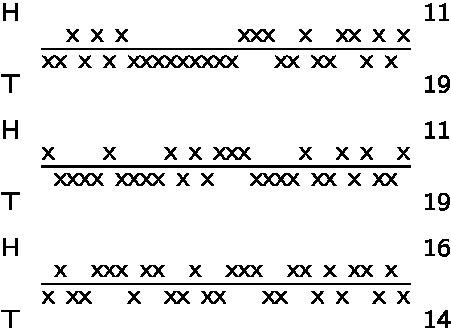
\includegraphics[width=0.8\linewidth]{fyz_fig0077.pdf}
      \caption{Pozorované posloupnosti hlava znaků ve třech hrách po třiceti hodech 
              (\cite[s.~79]{Feynman01})}
      \label{fyz:fig0077}
    \end{figure}
    Ve třech pokusech jsme ani jednou nedostali \num{15} hlav. Je to snad vinou mince? Nebo jsme se 
    zmýlili v úvaze vedoucí k závěru, že nejpravděpodobnější počet hlav v takové hře je \num{15}? 
    Abychom získali \num{100} experimentů, každý po \num{30} hodech, uskutečnili jsme dalších 
    \num{97} \uv{kol}. Výsledek experimentu ukazuje tab. \ref{fyz:fig0079}\footnote{Po prvních třech 
    hrách jsme experiment ve skutečnosti provedli tak, že jsme silně zatřásli krabicí, v níž bylo 
    \num{30} mincí a pak jsme spočetli všechny hlavy.}.
    
    Prohlédneme-li si čísla v tab. \ref{fyz:fig0079}, zjistíme, že většina výsledků je blízko čísla 
    \num{15} v tom smyslu, že se nacházejí mezi čísly \num{12} a \num{18}. K získání lepšího citu 
    pro chápání detailů těchto výsledků je vhodné zakreslit graf \emph{rozložení} výsledků. Určíme 
    počet her, v nichž jsme získali \(k\) hlav a znázorníme si je pro každé \(k\). Takový graf je 
    znázorněn na obr. \ref{fyz:fig0078}. \num{15} hlav jsme získali ve \num{13} hrách. \num{14} 
    hlav jsme získali \num{13}-krát. \num{16} i \num{17} hlav jsme získali dokonce více než 
    \num{13}-krát.

    \begin{figure}[ht!]  %\ref{fyz:fig0079}
      \centering
      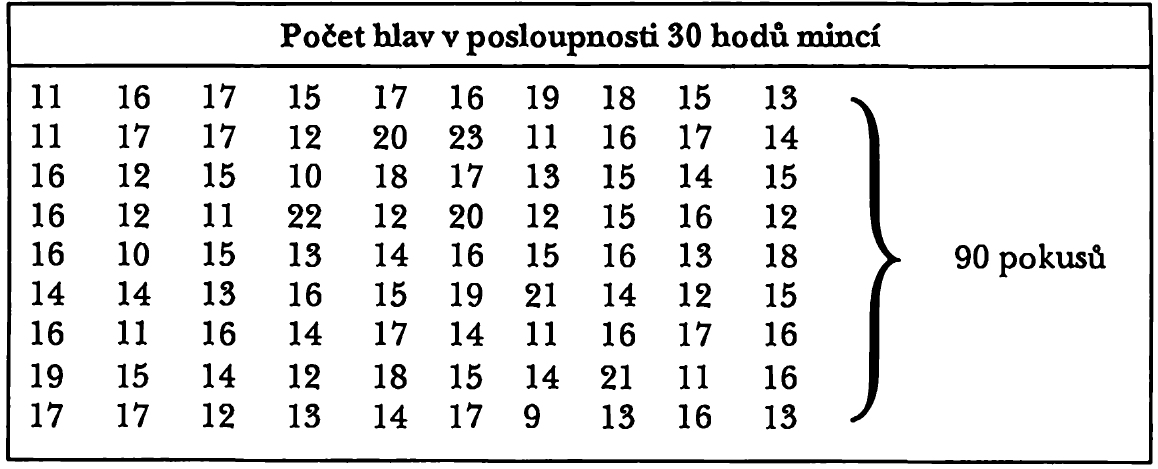
\includegraphics[width=1\linewidth]{fyz_fig0079.png}
      \caption{Tabulka počtu hlav v posloupnosti \num{30} hodů mincí (\cite[s.~80]{Feynman01})}
      \label{fyz:fig0079}
    \end{figure}
    Je možné z toho odvodit, že jde o jakousi zaujatost ve prospěch hlav? Nebyl náš „nejlepší 
    odhad“ dostatečně dobrý? Můžeme říci, že nejpravděpodobnější počet hlav pro jednu hru 
    sestávající z \num{30} hodů je \num{16}? Musíme být opatrní! Ve všech hrách se dohromady 
    uskutečnilo \num{3000} hodů. Hlav padlo celkem \num{1492}. Poměr počtu hlav k celkovému počtu 
    je tedy \num{0.497}, což je sice jen o málo, ale přece jen méně než polovina. Určitě tedy 
    nemůžeme předpokládat, že pravděpodobnost padnutí hlavy je větší než \num{0.5}! Skutečnost, že 
    v \emph{určité} sérii pozorování padne hlava nejčastěji \num{16}-krát, představuje 
    \emph{fluktuaci}. Jsme stále přesvědčeni, že \emph{nejpravděpodobnějším} počtem hlav je 
    \num{15}.
    
    Je možné položit otázku: Jaká pravděpodobnost, že hra s \num{30} hody dá \num{15}, \num{16} 
    nebo nějaký jiný počet hlav?“ Již jsme řekli, že při jednom hodu je pravděpodobnost pádu 
    \emph{jedné} hlavy \num{0.5} a i pravděpodobnost, že nepadne hlava, je \num{0.5}. Ve hře 
    sestávající ze dvou hodů máme \emph{čtyři} možné výsledky: \texttt{HH}, \texttt{HZ}, 
    \texttt{ZH}, \texttt{ZZ}. Protože každá z těchto posloupností je stejně pravděpodobná, můžeme 
    prohlásit, že
    \begin{enumerate}[noitemsep]
      \item pravděpodobnost padnutí dvou hlav je \num{1/4}, 
      \item pravděpodobnost padnutí jedné hlavy je \num{2/4}, 
      \item pravděpodobnost, že nepadne hlava je \num{1/4}. 
    \end{enumerate}
    Existují dva způsoby získávání jedné hlavy, ale jen jeden způsob získávání dvou hlav nebo žádné 
    hlavy.
    
    \begin{figure}[ht!]  %\ref{fyz:fig0078}
      \centering
      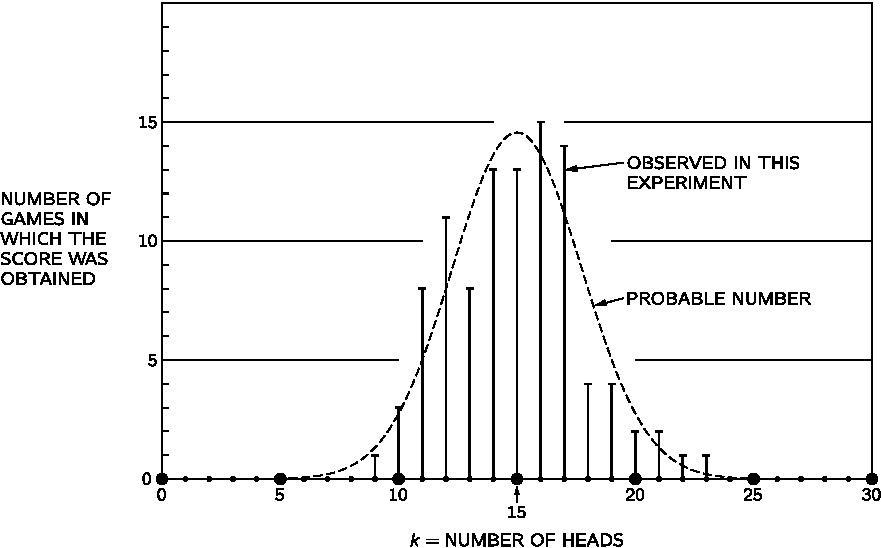
\includegraphics[width=1\linewidth]{fyz_fig0078.pdf}
      \caption{Souhrn výsledků l00 her po 30pokusech. Vertikální čáry ukazuj počty her,v nichž 
              padlo \(k\) hlav. Přerušovaná čára ukazuje očekávaný počet her, v nichž padne \(k\) 
              hlav, získaný výpočtem pravděpodobnosti (\cite[s.~80]{Feynman01})}
      \label{fyz:fig0078}
    \end{figure}
    
    Uvažujme nyní hru sestávající ze tří hodů. Pro třetí hod je stejně pravděpodobné, že padne 
    hlava nebo znak. Existuje jen jeden způsob získání tří hlav: v prvních dvou hodech 
    \emph{musely} padnout dvě hlavy a potom hlava i po třetím hodu. Existují však \emph{tři} 
    způsoby získání dvou hlav. Může padnout znak po padnutí dvou hlav (jeden způsob), nebo může 
    padnout hlava po padnutí jen jednoho znaku v prvních dvou hodech (dva způsoby). Tak pro možnosti
    \num{3}, \num{2}, \num{1}, \num{0} hlav existují \num{1}, \num{3}, \num{3}, \num{1} stejně 
    pravděpodobné způsoby představující celkově \num{8} různých posloupností. Příslušné 
    pravděpodobnosti jsou \num{1/8}, \num{3/8}, \num{3/8}, \num{1/8}.

    \begin{figure}[ht!]  %\ref{fyz:fig0081}
      \centering
      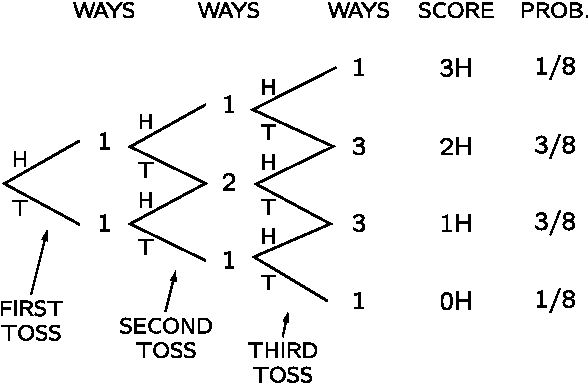
\includegraphics[width=1\linewidth]{fyz_fig0081.pdf}
      \caption{Diagram znázorňující počet různých způsobů padnutí \num{0}, \num{1}, \num{2} nebo 
              \num{3} hlav ve hře sestávající ze tří hodů (\cite[s.~81]{Feynman01})}
      \label{fyz:fig0081}
    \end{figure}
    
    To, co jsme řekli, je možno vyjádřit diagramem na obr. \ref{fyz:fig0081}. Je jasné, že takové 
    diagramy lze sestrojit i pro hry s vyšším počtem hodů. Obr. \ref{fyz:fig0080} znázorňuje takový 
    diagram pro hru se šesti hody. Počet způsobů odpovídajících libovolnému bodu diagramu je 
    vlastně počet různých cest (posloupností hlav a znaků), po nichž lze vyjít z počátečního bodu. 
    Počet úseků šikmo vzhůru udává počet vržených hlav. Soubor čísel, které se objevují v takovém 
    diagramu, je znám jako \textbf{Pascalův trojúhelník}. Čísla jsou známá i pod názvem 
    \emph{binomické koeficienty}, neboť se objevují i v rozvoji \((a + b)^n\). Označíme-li počet 
    hodů \(n\) a počet vržených hlav \(k\), pak se čísla vystupující v diagramu označují symbolem  
    \(\binom{n}{k}\). Bude vhodné připomenout, že binomické koeficienty 
    lze vypočítat ze vztahu
    \begin{equation}\label{fyz:eq074}
      \binom{n}{k} = \frac{n!}{k!(n-k)!}.
    \end{equation}
    kde \(n!\), nazývaný „n-faktoriál“, představuje součin \(n(n- 1)(n-2)\cdots (3)(2)(1)\).
    
    \begin{figure}[ht!]  %\ref{fyz:fig0080}
      \centering
      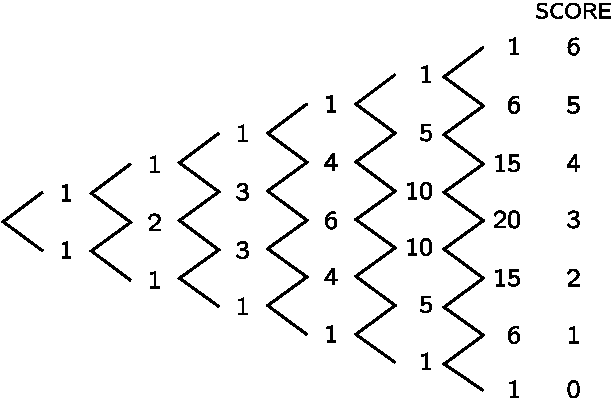
\includegraphics[width=1\linewidth]{fyz_fig0080.pdf}
      \caption{Diagram jako na obr. \ref{fyz:fig0081}, ale pro hru sestávající ze \num{6} hodů
               (\cite[s.~82]{Feynman01})}
      \label{fyz:fig0080}
    \end{figure}
    
    Nyní již můžeme počítat pravděpodobnosti \(P(k, n)\) toho, že při \(n\) hodech padne hlava,
    pomocí definice (\ref{fyz:eq069}). Celkový počet možných posloupností je \(2^n\) (neboť každý
    hod připouští 2 výsledky) a počet způsobů získání \(k\) hlav je \(\binom{n}{k}\), přičemž
    všechny jsou stejně pravděpodobné. Proto máme
    \begin{equation}\label{fyz:eq075}
      P(k,n) = 
      \frac{\binom{n}{k}}{2^n}.
    \end{equation}
    
    Protože \(P(k, n)\) je podíl her, při nichž očekáváme, že padne \(k\) hlav, lze pak očekávat, 
    že při \num{100} hrách padne \(k\) hlav \(100\cdot P(k, n)\) krát. Přerušovaná čára na obr. 
    \ref{fyz:fig0078} prochází body vypočítanými ze vztahu \(100\cdot P(k, 30)\). Vidíme, že padnutí 
    \num{15} hlav jsme \emph{očekávali ve} \num{14} nebo \num{15} hrách, zatímco tato událost byla 
    pozorována ve \num{13} hrách. Padnutí \num{16} hlav jsme \emph{očekávali ve} \num{13} nebo 
    \num{14} hrách, ale \num{16} hlav padlo v \num{16} hrách. Takové fluktuace jsou „součástí hry“.
    
    Použitou metodu je možné aplikovat i na tu nejobecnější situaci, v níž jsou jen dva možné 
    výsledky jednoho pozorování. Označme tyto dva výsledky \(V\) („výhra“) a \(P\) („prohra“). V 
    obecném případě pravděpodobnosti výsledku \(V\) nebo \(P\) u jedné události nemusí být stejné. 
    Označme \(p\) pravděpodobnost výhry \(V\). Potom \(q\), pravděpodobnost prohry, musí být nutně 
    \((1 - p)\). V souboru \(n\) pokusů je pravděpodobnost \(P(k, n)\) toho, že vyhrajeme 
    \(k\)-krát rovna
    \begin{equation}\label{fyz:eq076}
      \boxed{P(k,n) = \binom{n}{k}p^kq^{n-k}}\,.
    \end{equation}
    Tato pravděpodobnostní funkce se nazývá \textbf{Bernoulliho} nebo i \textbf{binomickou 
    pravděpodobností}.
    
  \section{Náhodná procházka}
    Existuje další zajímavý problém, v němž vystupuje myšlenka pravděpodobnosti. Je to problém 
    \emph{„náhodné procházky“}. Jako nejjednodušší verzi této úlohy si představme „hru“, v níž 
    „hráč“ startuje v bodě \(x = 0\) a při každém tahu má udělat krok \emph{buď} dopředu (směrem 
    \(k + x\)) nebo dozadu (směrem \(k - x\)). Volba se má uskutečnit náhodně, například pomocí 
    hodu mincí. Jak popíšeme výsledný pohyb? Ve své obecné formě se problém vztahuje na pohyb atomů 
    (nebo jiných částic) v plynech - jde o \textbf{Brownův pohyb} - a i na kombinaci chyb při 
    měřeních. Uvidíme, že problém náhodné procházky úzce souvisí s problémem házení mincí, o němž 
    jsme již hovořili.

    \begin{figure}[ht!]  %\ref{fyz:fig0082}
      \centering
      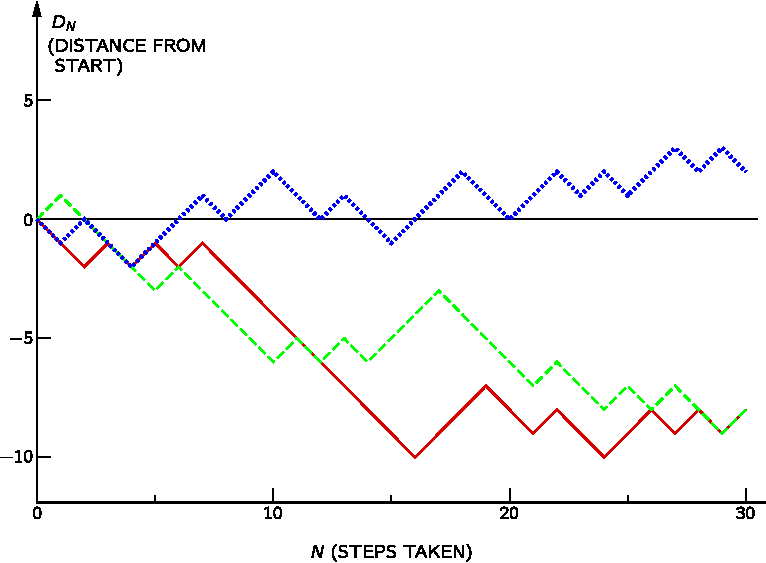
\includegraphics[width=1\linewidth]{fyz_fig0082.pdf}
      \caption{Postup náhodné procházky. Horizontální souřadnice \(N\) představuje celkový počet 
               kroků: vertikální souřadnice \(D(N)\) představuje vzdálenost, do níž se chodec 
               dostal z počátečního bodu. (\cite[s.~83]{Feynman01})}
      \label{fyz:fig0082}
    \end{figure}
    
    Nejprve si všimněme několika příkladů náhodné procházky. Postup chodce můžeme charakterizovat 
    čistou vzdáleností \(D_N\) ušlou v \(N\) krocích. Na obr. \ref{fyz:fig0082} jsou vidět tři 
    příklady dráhy náhodného chodce. (Jako náhodné posloupnosti volby kroků jsme použili výsledky 
    házení mincí z obr. \ref{fyz:fig0077}.)
    
    Co je možné říci o takovém pohybu? Především se můžeme ptát: Jak daleko se chodec v průměru 
    dostane?“ Musíme \emph{očekávat}, že jeho průměrný postup bude nulový, protože se stejně 
    pravděpodobně dostává dopředu nebo dozadu. Máme však takový pocit, že čím více \(N\) roste, tím 
    je pravděpodobnější, že chodec zabloudí dále od počátku. Proto se můžeme ptát, jaká je jeho 
    průměrná ušlá vzdálenost v \emph{absolutní hodnotě}, tj. jaký je průměr z \(\abs{D}\). Je však 
    výhodnější pracovat s jinou mírou „postupu“, se čtvercem vzdálenosti: \(D^2\) je kladné pro 
    kladný i záporný pohyb, a je proto vhodnou \emph{mírou} takového náhodného putování.
    
    Je možné dokázat, že očekávaná hodnota \(D_N^2\) je právě \(N\), tedy počet absolvovaných 
    kroků. „Očekávanou hodnotou“ rozumíme pravděpodobnou hodnotu (náš nejlepší odhad), kterou 
    můžeme považovat za \emph{očekávané} průměrné chování v mnoha opakovaných posloupnostech. 
    Takovou očekávanou hodnotu označujeme i \(\left\langle D_N^2\right\rangle\) a nazýváme ji i 
    \textbf{střední hodnotou čtverce vzdálenosti}. Po jednom kroku je \(D^2\) určitě rovno \(+1\), 
    máme tedy určitě \(\left\langle D_1^2\right\rangle = 1\). (Všechny vzdálenosti budou měřeny 
    tak, aby krok představoval jednotku. Jednotky vzdálenosti už nebudeme psát).

    Očekávanou hodnotu  \(\left\langle D_N^2\right\rangle\) pro \(N>1\) lze získat z \(D_{N-1}\). 
    Jestliže po \(N - 1\) krocích máme \(D_{N-1}\), pak po \(N\) krocích máme \(D_N = D_{N-1} + 1\) 
    nebo \(D_N = D_{N-1} - 1\). Pro druhé mocniny platí
    
    \begin{equation}\label{fyz:eq077}
      D_N^2 = 
        \begin{cases}
          D^2_{N-1} + 2D_{N-1} + 1 \\
          \quad\text{nebo}        \\
          D^2_{N-1} - 2D_{N-1} + 1
        \end{cases}
    \end{equation}
    Máme-li řadu nezávislých posloupností, očekáváme, že každá z těchto hodnot se objeví v polovině 
    případů, tedy naše průměrné očekávání je právě průměr ze dvou možných hodnot. Očekávaná hodnota 
    \(D_N\) je tedy \(D^2_{N-1} + 1\). Obecně můžeme očekávat pro \(D^2_{N-1}\) „očekávanou 
    hodnotu“  \(\left\langle D_{N-1}^2\right\rangle\) (podle definice !). Proto máme
    \begin{equation}\label{fyz:eq078}
      \left\langle D_N^2\right\rangle = \left\langle D_{N-1}^2\right\rangle + 1.
    \end{equation}
    Již jsme viděli, že \(\left\langle D_1^2\right\rangle = 1\) a proto musí být
    \begin{equation}\label{fyz:eq079}
      \left\langle D_N^2\right\rangle = N.
    \end{equation}
    Dostali jsme tedy velmi jednoduchý výsledek!
    
    Kdybychom při náhodné procházce chtěli „postup od začátku“ charakterizovat vzdáleností a ne 
    čtvercem vzdálenosti, museli bychom použít „střední kvadratickou vzdálenost“ \(D_{\text{stř}}\)
    \begin{equation}\label{fyz:eq080}
      D_{\text{stř}} = \sqrt{\left\langle D^2\right\rangle} = \sqrt{N}.
    \end{equation}
    
    Již jsme řekli, že náhodná procházka je z matematického hlediska velmi podobná hře házení 
    mincí, kterou jsme uvažovali na začátku kapitoly. Uvědomíme-li si, že směr každého kroku je v 
    souladu s padnutím hlavy nebo znaku ve hře s mincí, pak \(D\) je právě \(N_H - N_Z\), tedy 
    rozdíl počtu hlav a znaků. Protože je \(N_H + N_Z = N,\) kde \(N\) je celkový počet kroků (a 
    tedy i hodů), pak máme \(D = 2 N_H - N\). Již dříve jsme odvodili výraz pro očekávané rozdělení 
    \(N_H\) (nazývané i \(k\)) a dostali jsme výsledek (\ref{fyz:eq075}). Protože \(N\) je 
    konstanta, máme vlastně rozdělení odpovídající \(D\). (Protože pro každou hlavu navíc proti 
    \(N/2\) „chybí“ znak, máme faktor \(2\) mezi \(N_H\) a \(D\)). Grafy na obr. \ref{fyz:fig0078} 
    představují rozdělení vzdáleností, jichž můžeme dosáhnout třiceti náhodnými kroky (kde \(k = 
    15\) znamená \(D = 0\), \(k= 16\), \(D = 2\) atd.).
    
    Odchylka \(N_H\) od očekávané hodnoty \(N/2\) je
    \begin{equation}\label{fyz:eq081}
      N_H - \frac{N}{2} = \frac{D}{2}
    \end{equation}
    a dále pro střední kvadratickou odchylku máme
    \begin{equation}\label{fyz:eq082}
      \left(N_H - \frac{N}{2}\right)_\text{stř} = \frac{1}{2}\sqrt{N}.
    \end{equation}
    
    V souladu s výsledky, které jsme získali pro \(D_{\text{stř}}\), očekáváme, že „typická“ 
    vzdálenost při třiceti krocích by měla být \(\sqrt{30} = \num{5.5}\), tedy typické \(k\) by 
    mělo být přibližně \(\num{5.5}/2 = \num{2.8}\) jednotek z \num{15}. Vidíme, že „šířka“ křivky 
    na obr. \ref{fyz:fig0078} měřená od středu je přibližně \num{3} jednotky, což souhlasí s tímto 
    výsledkem.
    
    Dostali jsme se už tak daleko, že se můžeme zabývat otázkou, které jsme se dosud vyhýbali. Jak 
    můžeme rozhodnout, je-li mince „poctivá“ nebo „falešná“? Nyní můžeme na tuto otázku odpovědět 
    alespoň částečně. V případě poctivé mince očekáváme, že hlava se objeví v polovině případů, tj.
    \begin{equation}\label{fyz:eq083}
      \frac{\left\langle N_H\right\rangle}{N} = \num{0.5}.
    \end{equation}
    Očekáváme také, že skutečné \(N_H\) se bude lišit od \(N/2\) přibližně o \(\sqrt{N/2}\), nebo, 
    že podíl se bude lišit o
    \begin{equation}\label{fyz:eq084}
      \frac{1}{N}\cdot\frac{\sqrt{N}}{2} = \frac{1}{2\sqrt{N}}.
    \end{equation}
    Čím je \(N\) větší, tím blíže k jedné polovině bude podle našeho očekávání podíl \(N_H/N\).
    
    Na obr. \ref{fyz:fig0083} je vynesen podíl \(N_H/N\) pro výše uvedenou hru s mincí. Z obrázku je 
    zřejmá snaha tohoto podílu dosáhnout hodnoty \num{0.5} při velkých \(N\). Naneštěstí pro žádnou 
    konkrétní hru nebo kombinaci her neexistuje \emph{záruka}, že pozorovaná odchylka bude alespoň 
    \emph{blízko očekávané odchylky}. Vždy existuje konečná možnost, že velká fluktuace - dlouhá 
    řada hlav nebo znaků způsobí libovolně velkou odchylku. Můžeme říci jen to, že v případě 
    odchylky, která se jen málo liší od hodnoty \(1/2\sqrt{N}\) (řekněme v rozsahu faktoru \num{2} 
    nebo \num{3}), nemáme důvod podezřívat minci z nepoctivosti. Je-li odchylka mnohem větší, může 
    vzniknout nedokazatelné podezření, že mince je upravena (nebo že hráč je příliš šikovný!).
    
    \begin{figure}[ht!]  %\ref{fyz:fig0083}
      \centering
      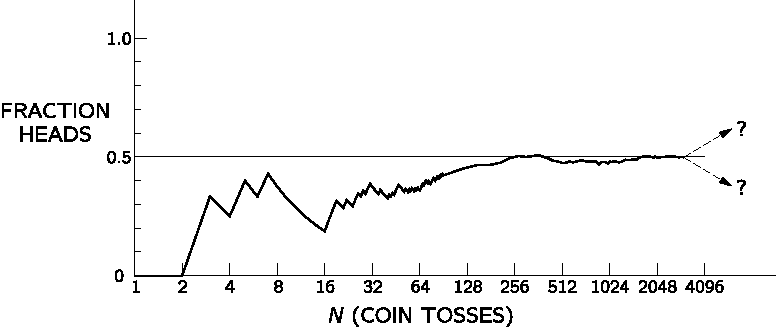
\includegraphics[width=1\linewidth]{fyz_fig0083.pdf}
      \caption{Podíl hodů, v nichž padla hlava v určité posloupnosti \(N\) hodů mincí  
               (\cite[s.~85]{Feynman01})}
      \label{fyz:fig0083}
    \end{figure}
    
    Nehovořili jsme ani o tom, co dělat v tom případě, kdy máme vážný důvod předpokládat, že 
    „mince“ nebo podobný jiný „náhodně“ se chovající předmět (například plochý kámen, který může 
    dopadnout jen na jednu nebo druhou stranu) \emph{budou mít} různé pravděpodobnosti, že padne 
    hlava nebo znak. Definovali jsme \(P(H) =\left\langle N_H\right\rangle/N\). Jak se dozvíme, co 
    je možné \emph{očekávat} pro \(N_H\). To nejlepší, co je možné v některých případech udělat, je 
    pozorovat počty hlav, které padnou při velkém počtu hodů. Z nedostatku lepší možnosti, musíme 
    položit \(\left\langle N_H\right\rangle = N_H\) (pozorované). (Co jiného je možné očekávat?) 
    Musíme si však uvědomit, že v takovém případě různé experimenty nebo různí pozorovatelé mohou 
    stanovit jinou hodnotu \(P(H)\). Je však možné \emph{očekávat}, že tyto hodnoty by se měly 
    lišit nejvýše odchylkou \(1/2\sqrt{N_H}\), je-li \(P(H)\) blízko \num{0.5}. Experimentální 
    fyzik říká, že „experimentálně určená“ pravděpodobnost má „chybu“ a píše
    \begin{equation}\label{fyz:eq085}
      P(H) = \frac{N_H}{N}\pm\frac{1}{2\sqrt{N}}.
    \end{equation}
    
    U takového výrazu se předpokládá, že \emph{existuje} „pravdivá“ nebo „správná“ pravděpodobnost, 
    kterou by bylo možné vypočítat, kdybychom toho dost věděli, a že pozorování mohou být zatížena 
    „chybou“ následkem fluktuace. Takovýto předpoklad však není možné logicky zdůvodnit. Je snad 
    lepší si uvědomit, že pojem pravděpodobnosti je svým způsobem subjektivní, že je vždy založen 
    na nejistých poznatcích a že jeho kvantitativní vyjádření podléhá změnám při získávání dalších 
    informací.
        
  \section{Rozložení pravděpodobnosti}
    Vraťme se opět k náhodné procházce a uvažujme o její obměně. Předpokládejme, že kromě náhodné 
    volby \emph{směru} (+ nebo -) každého kroku se mění i \emph{délka} kroku nějakým 
    nepředvídatelným způsobem, přičemž jedinou podmínkou je to, že v \emph{průměru} je délka kroku 
    jednotková. Takovýto případ lépe vystihuje něco takového, jako je tepelný pohyb molekul v 
    plynu. Je-li \(S\) délka kroku, pak \(S\) může dosáhnout jakékoli hodnoty, ale nejčastěji bude 
    \uv{blízko} \num{1}. Konkrétně budiž \(\left\langle S^2\right\rangle = 1\), nebo, což je totéž 
    \(S_{\text{stř}} = 1\). Při odvozování \(\left\langle D^2\right\rangle\) budeme postupovat jako 
    předtím, s tím rozdílem, že rovnice (\ref{fyz:eq078}) se nyní změní na
    \begin{equation}\label{fyz:eq086}
      \left\langle D_N^2\right\rangle 
        = \left\langle D_{N-1}^2\right\rangle + \left\langle s^2\right\rangle
        = \left\langle D_{N-1}^2\right\rangle + 1.
    \end{equation}
    Stejně jako předtím, i nyní dostaneme
    \begin{equation}\label{fyz:eq087}
      \left\langle D_N^2\right\rangle = N.
    \end{equation}
    Jaké bude nyní rozložení vzdáleností \(D\). Jaká je například pravděpodobnost toho, že \(D = 
    0\) po \num{30} krocích? Taková pravděpodobnost je nulová! Pravděpodobnost, že \(D\) bude 
    \emph{libovolná daná} hodnota, je nulová, neboť je zcela nepravděpodobné, že by součet všech 
    zpětných kroků (různých délek) byl přesně stejný jako součet kroků vpřed. Nemůžeme sestrojit 
    takový graf jako na obr. \ref{fyz:fig0078}.
    
    Podobné znázornění jako na obr. \ref{fyz:fig0078} je však možné, neptáme-li se na 
    pravděpodobnost \(D\) rovného přesně \num{0.1} nebo \num{2}, ale jestliže se zajímáme o 
    pravděpodobnost \(D\) \emph{v blízkosti} \num{0.1} nebo \num{2}. Definujme \(P(x, \Delta x)\) 
    jako pravděpodobnost toho, že \(D\) bude ležet v intervalu šířky \(\Delta x\) v okolí bodu 
    \(x\) (například od \(x\) po \(x + \Delta x\)). Očekáváme, že pro malé \(\Delta x\) je 
    pravděpodobnost toho, že \(D\) bude ležet v tomto intervalu, úměrná \(\Delta x\), tj. šířce 
    intervalu. Můžeme proto psát
    \begin{equation}\label{fyz:eq088}
      P(x,\Delta x) = p(x)\Delta x.
    \end{equation}
    Funkci \(p(x)\) nazýváme \textbf{hustotou pravděpodobnosti}.
    
    Tvar \(p(x)\) závisí na počtu kroků \(N\) i na rozdělení jednotlivých délek kroků. Nemůžeme to 
    zde dokazovat, ale pro velké \(N\) je hustota \(p(x)\) stejná pro všechna rozumná rozdělení 
    jednotlivých délek kroků a závisí jen na \(N\). Na obr. \ref{fyz:fig0084} je znázorněno \(p(x)\) 
    pro tři hodnoty \(N\). Všimněte si, že pološířky těchto křivek (jejich rozšíření na úrovni 
    poloviny maximální výšky) jsou \(\sqrt{N})\) v souladu s našimi předcházejícími úvahami.
    
    Dále si můžeme všimnout, že hodnota \(p(x)\) v blízkosti nuly je nepřímo úměrná \(\sqrt{N}\). 
    Je tomu tak proto, že všechny křivky mají podobný tvar a plochy pod křivkami musí být stejné. 
    Protože \(p(x)\Delta x\) je pravděpodobnost nalezení \(D\) v \(\Delta x\) při malých hodnotách 
    \(\Delta x\), můžeme určit pravděpodobnost toho, že \(D\) se nachází někde uvnitř libovolného 
    intervalu ohraničeného body \(x_1\), \(x_2\) tak, že tento interval rozdělíme na malé části 
    \(\Delta x\) a vypočteme součet členů \(p(x)\Delta x\) pro každou takovou část.     
    Pravděpodobnost, že \(D\) se nachází někde mezi \(x_1\) a \(x_2\), což můžeme zapsat \(P(x_1 < 
    D < x_2)\), je rovna obsahu vyšrafované oblasti na obr. \ref{fyz:fig0085}. Čím menší jsou 
    přírůstky \(\Delta x\), tím přesnější bude výsledek. Proto můžeme napsat, že
    \begin{equation}\label{fyz:eq089}
      P(x_1 < D < x_2) = \sum p(x)\Delta x = \int_{x_1}^{x_2}p(x)dx.
    \end{equation}
    Obsah plochy pod celou křivkou je pravděpodobnost, že \(D\) se někde nachází (tj. má nějakou 
    hodnotu mezi \(x=-\infty\) a  \(x= +\infty\)).

    \luagraphic[1]{fyz_fig0084.pdf}{Hustota pravděpodobnosti dosažení vzdálenosti \(D\) od počátku
    při náhodné procházce sestávající z \(N\) kroků (\(D\) se měří v jednotkách střední kvadratické
    délky kroku) (\cite[s.~87]{Feynman01})}{fyz:fig0084}
      
    Tato pravděpodobnost je rovna \(1\). Musí tedy být
    \begin{equation}\label{fyz:eq090}
      \int_{-\infty}^{\infty}p(x)dx = 1.
    \end{equation}
    
    Protože křivky na obr. \ref{fyz:fig0084} se rozšiřují úměrně \(\sqrt{N}\), musí být jejich výška 
    úměrná \(1\sqrt{N}\), aby se zachoval celkový obsah plochy rovný \num{1}.

    \begin{figure}[ht!]  %\ref{fyz:fig0084}
      \centering
      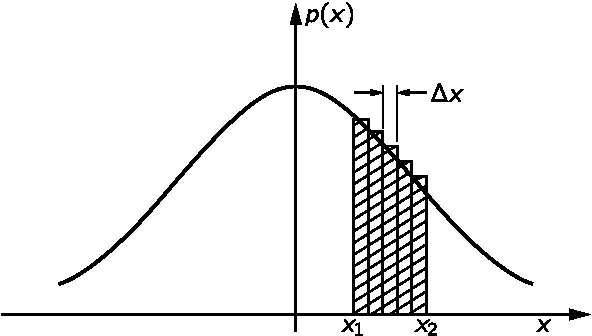
\includegraphics[width=1\linewidth]{fyz_fig0085.pdf}
      \caption{Pravděpodobnost, že při náhodné procházce se ušlá vzdálenost \(D\) nachází mezi 
                body  \(x_1\) a \(x_2\), je dána obsahem plochy pod křivkou \(p(x)\) mezi \(x_1\) a 
                \(x_2\).
                \cite[s.~87]{Feynman01}}
       \label{fyz:fig0085}
    \end{figure}
    
    S hustotou pravděpodobnosti, o níž jsme právě hovořili, se setkáváme nejčastěji. Je známá jako 
    \textbf{normální} nebo \textbf{Gaussova hustota pravděpodobnosti}. Její matematický zápis je
    \begin{equation}\label{fyz:eq091}
      p(x) = \frac{1}{\sigma\sqrt{2\pi}}e^{-\frac{x^2}{2\sigma^2}},	
    \end{equation}    
    přičemž veličina \(\sigma\) se nazývá \emph{standardní odchylkou}. V našem případě je \(\sigma 
    = \sqrt{N}\), nebo je-li střední kvadratická délka kroku různá od \num{1}, je 
    \(\sigma=\sqrt{N}S_\text{stř}\).
    
    Již jsme uvedli, že pohyb molekuly nebo každé jiné částice v plynu je podobný náhodné 
    procházce. Předpokládejme, že otevřeme láhev s organickou sloučeninou a necháme část její páry 
    uniknout do vzduchu. Existuje-li proudění vzduchu, tak že vzduch cirkuluje, budou unášeny i 
    uvedené páry. Jenže i v dokonale klidném vzduchu se budou páry postupně rozptylovat - 
    difundovat - dokud neproniknou do celé místnosti. Můžeme je registrovat podle jejich barvy nebo 
    zápachu. Jednotlivé molekuly organických par se šíří i v klidném vzduchu v důsledku 
    molekulárního pohybu způsobovaného srážkami s jinými molekulami. Známe-li délku „kroku“ a počet 
    kroků za sekundu, můžeme zjistit pravděpodobnost, v jaké vzdálenosti od svého původního místa 
    se ocitne po určitém čase jedna nebo několik molekul. Postupem času počet kroků roste a plyn se 
    rozplývá tak, jak je znázorněno křivkami na obr. \ref{fyz:fig0084}. V jedné z dalších kapitol 
    určíme, jak závisí délka a frekvence kroků na teplotě a tlaku plynu.
    
    Již jsme hovořili o tom, že tak plynu je následkem srážek molekul se stěnami nádoby. Až později 
    přejdeme ke kvantitativnímu popisu tohoto jevu, musíme znát rychlost molekul narážejících na 
    stěnu, protože síla jejich nárazu závisí na rychlosti. Nemůžeme však hovořit o \emph{určité} 
    rychlosti molekul. Tento děj můžeme popsat jen pomocí pravděpodobností. Molekula může mít 
    jakoukoli rychlost, ale některé rychlosti jsou pravděpodobnější než jiné. Procesy probíhající v 
    plynu můžeme popsat pomocí pravděpodobnosti \(p(v)\Delta v\), že daná molekula má rychlost z 
    intervalu \(v, v+ \Delta v\). Hustota pravděpodobnosti \(p(v)\) je přitom funkcí rychlosti 
    \(v\). Později se dozvíte, jak Maxwell využitím zdravého rozumu a myšlenek teorie 
    pravděpodobnosti našel matematické vyjádření funkce \(p(v)\). Tvar\footnote{Maxwellův výraz je 
    \(p(v) = Cv^2e^{-av^2}\), kde \(a\) je konstanta související s teplotou a \(C\) je zvoleno tak, 
    aby celková pravděpodobnost byla rovna jedné.} funkce \(p(v)\) je znázorněn na obr. 
    \ref{fyz:fig0086}. Rychlost může dosáhnout libovolné hodnoty, ale s největší pravděpodobností 
    bude blízká nejpravděpodobnější nebo očekávané hodnotě \(\langle v\rangle\)).
    
    \begin{figure}[ht!]  %\ref{fyz:fig0086}
      \centering
      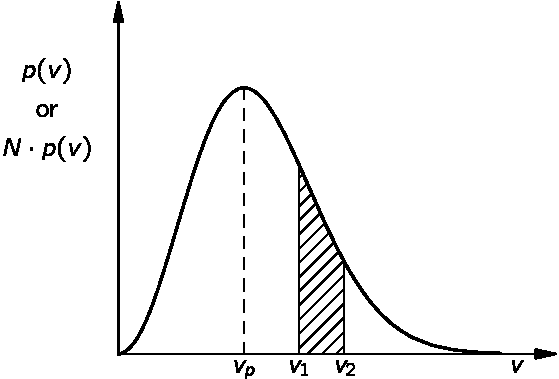
\includegraphics[width=1\linewidth]{fyz_fig0086.pdf}
      \caption{Rozložení rychlosti molekul plynu  (\cite[s.~88]{Feynman01})}
      \label{fyz:fig0086}
    \end{figure}
    
    O křivce znázorněné na obr, \ref{fyz:fig0086} často uvažujeme trochu jinak. Máme-li molekuly 
    plynu uzavřené v typické nádobě (která má objem např. \SI{1}{\litre}), jde vlastně o velmi 
    velké množství \(N\) molekul (\(N\approx\num{e22}\)). Protože \(p(v)\Delta v\) je 
    pravděpodobnost toho, že \emph{jedna} molekula bude mít rychlost z intervalu \(\Delta v\), pak 
    podle naší definice pravděpodobnosti bude \emph{očekávaný} počet molekul \(\langle N\rangle\) s 
    rychlostmi z intervalu \(\Delta v\)
    \begin{equation}\label{fyz:eq092}
      \langle N\rangle = Np(v)\Delta v.
    \end{equation}
    Veličinu \(Np(v)\) proto nazýváme „\emph{rozdělením molekul podle rychlosti}“. Plocha pod 
    křivkou mezi dvěma hodnotami rychlosti \(v_1\) a \(v_2\), např. vyšrafovaná plocha na obr. 
    \ref{fyz:fig0086}, představuje (v případě křivky \(Np(v)\)) očekávaný počet molekul s rychlostmi 
    mezi \(v_1\) a \(v_2\). Protože v případě plynu máme obvykle co činit s velkým počtem molekul, 
    předpokládáme malé odchylky od očekávaných hodnot (jako \(1/\sqrt{N}\)), a proto často 
    vynecháváme slovo „očekávaný“ a říkáme: „Počet molekul s rychlostmi mezi \(v_1\) a \(v_2\) 
    odpovídá obsahu příslušné plochy pod křivkou.“ Nesmíme však zapomenout, že takové výroky se 
    vždy týkají \emph{pravděpodobných} počtů.
    
  \section{Princip neurčitosti}
    Myšlenky pravděpodobnosti jsou jisté užitečné při popisu chování řádově \num{e22} molekul v 
    plynu, protože již samotný pokus o určení polohy nebo rychlosti každé molekuly by byl úžasně 
    nepraktický. Když se poprvé na takový problém aplikovala teorie pravděpodobnosti, chápalo se to 
    jako \emph{vhodný} způsob popisu tak složitých situací. Dnes jsme však toho názoru, že idea 
    pravděpodobnosti je při popisu atomových dějů \emph{nevyhnutelná}. Podle kvantové mechaniky, 
    matematické teorie částic, existuje vždy jistá nepřesnost při \emph{určení} poloh a rychlostí. 
    V nejlepším případě můžeme říci, že existuje jistá pravděpodobnost toho, že částice se bude 
    nacházet v blízkosti určitého bodu \(x\).
    
    Hustotu pravděpodobnosti \(p_1(x)\) udáme tak, že \(p_1(x)\Delta x\) představuje 
    pravděpodobnost výskytu částice mezi \(x\) a \(x+ \Delta x\). Je-li částice dostatečně dobře 
    lokalizovaná, např. v blízkosti \(x_1\), bude mít funkce \(p_1(x)\) průběh podobný grafu na 
    obr. \ref{fyz:fig0087a}. Podobně musíme určit rychlost částice pomocí hustoty pravděpodobnosti 
    \(p_2(v)\), přičemž \(p_2(v)\Delta v\) je pravděpodobnost toho, že rychlost je v intervalu mezi 
    \(v\) a \(v+\Delta v\).
    
    \begin{figure}[ht!]  %\ref{fyz:fig0087}
      \centering
      \subcaptionbox{\label{fyz:fig0087a}}{\luafigure[0.70]{fyz_fig0087a.pdf}}              \\
      \subcaptionbox{\label{fyz:fig0087b}}{\luafigure[0.70]{fyz_fig0087b.pdf}}
      \caption{Hustota pravděpodobnosti pozorování polohy a rychlosti částice  
               (\cite[s.~89]{Feynman01})}
      \label{fyz:fig0087}
    \end{figure}
    
    Jeden ze základních výsledků kvantové mechaniky spočívá v tom, že funkce \(p_1(x)\) a 
    \(p_2(v)\) není možné vybrat nezávisle, zejména nemohou být obě dvě libovolně úzké. Označíme-li 
    charakteristickou „šířku“ křivky \(p_1(x)[\Delta x]\) a křivky \(p_2(v)\) zase \([\Delta v]\), 
    jak je ukázáno na obrázku, potom příroda vyžaduje, aby \emph{součin} těchto šířek nebyl menší 
    než číslo \(h/m\), kde \(m\) je hmotnost částice a \(h\) je základní fyzikální konstanta zvaná 
    \textbf{Planckova konstanta}. Tento základní vztah je možné zapsat ve tvaru
    \begin{equation}\label{fyz:eq093}
      [\Delta x][\Delta v]\geq\frac{h}{m}.
    \end{equation}
    Tato rovnice je matematickým vyjádřením \textbf{Heisenbergova principu neurčitosti}, o němž 
    jsme se již zmínili.
    
    Protože pravá strana rovnice (\ref{fyz:eq093}) je konstantní, pak, „přinutíme-li“ částici 
    zaujmout určité místo, skončí to tím, že velmi vzroste její rychlost. Nebo přinutíme-li částici 
    pohybovat se velmi pomalu, nebo velmi přesnou rychlostí, „rozplyne se“, takže nebudeme umět 
    říci, kde se přesně nachází. Částice se chovají velmi podivně!
    
    Princip neurčitosti vyjadřuje přirozenou nejasnost, která musí existovat při každém pokusu 
    popsat přírodu. Náš nejpřesnější popis přírody musí byt v řeči \emph{pravděpodobnosti}.Jsou 
    však lidé, kteří se neumějí smířit s takovýmto popisem přírody. Domnívají se, že kdybychom 
    věděli, co se s částicí  \emph{skutečně} děje, mohli bychom znát současně její přesnou rychlost 
    a polohu. Na začátku rozvoje kvantové mechaniky tento problém velmi znepokojoval Einsteina. 
    Často potřásal hlavou a říkal \uv{Vždyť bůh neháže kostkou, aby rozhodl, jak se má pohybovat 
    elektron!} Dlouho se trápil s tímto problémem a pravděpodobně se nikdy nesmířil se skutečnosti, 
    že je to ten nejlepší popis přírody, který dokážeme udělat. Několik málo fyziků se ještě stále 
    zabývá tímto problémem doufajíce, že svět je možné popsat nějak jinak a vyloučit neurčitost v 
    chování částic. Zatím však v tomto směru nikdo nebyl úspěšný. 
    
    Nevyhnutelná neurčitost při určování polohy částice nabývá významu tehdy, když chceme popsat 
    strukturu atomů. V atomu vodíku, jenž má jádro skládající se z jednoho protonu a mimo jádro má 
    jeden elektron, je neurčitost v poloze elektronu tak velká jako atom samotný! Proto nemůžeme 
    dost dobře hovořit o elektronu pohybujícím se po určité dráze kolem protonu. Nanejvýš můžeme 
    říci, že existuje určitá pravděpodobnost \(p(r)\Delta V\) pozorování elektronu v elementu 
    objemu \(\Delta V\) ve vzdálenosti \(r\) od protonu. Hustota pravděpodobnosti \(p(r)\) udává 
    kvantová mechanika. Pro neporušený vodíkový atom je \(p(r) = Ae^{-\frac{r^2}{a^2}}\), což 
    představuje funkci se zvonovitým grafem podobnou funkci na obr. \ref{fyz:fig0085}. Číslo \(a\) 
    představuje \uv{charakteristický} poloměr, za nímž funkce rychle klesá. Protože je malá 
    pravděpodobnost výskytu elektronu ve větších vzdálenostech od jádra než \(a\), můžeme \(a\) 
    považovat za \uv{poloměr atomu}, což je asi \num{e-10} metru. 

    \begin{figure}[ht!]  %\ref{fyz:fig0088}
      \centering
      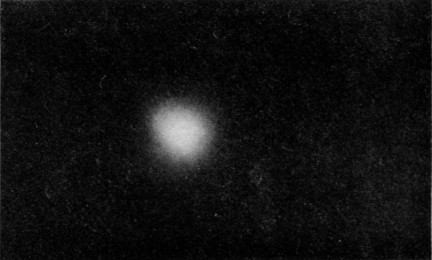
\includegraphics[width=0.8\linewidth]{fyz_fig0088.jpg}
      \caption{Způsob znázornění atomu vodíku. Hustota (bělost) oblaku představuje hustotu 
               pravděpodobnosti výskytu elektronu. 
               (\cite[s.~90]{Feynman01})}
      \label{fyz:fig0088}
    \end{figure}
    Představu o atomu vodíku můžeme získat, znázorníme-li si oblak, jehož hustota je úměrná hustotě 
    pravděpodobnosti výskytu elektronu. Příklad takového oblaku je na obr. \ref{fyz:fig0088}. Naší 
    nejlepší \uv{představou} vodíkového atomu je tedy jádro obklopené \uv{elektronovým oblakem} (ve 
    skutečnosti však máme na mysli \uv{oblak pravděpdobnosti}). Elektron je někde tam, ale příroda 
    nám dovoluje poznat jen \emph{pravděpodobnost} jeho výskytu na určitém místě.
    
    Ve svém úsilí po co nejúplnějším poznání přírody dospěla moderní fyzika poznání, že jisté věci 
    není možné \uv{poznat} s jistotou. Mnohé z našich poznatků vždy zůstanou nejisté. Nanejvýš 
    můžeme znát jejich pravděpodobnosti. 
    
  \section{Příklady a cvičení}
  
%} %tikzset
%---------------------------------------------------------------------------------------------------